\documentclass[a4paper, 12pt]{article}%тип документа



%отступы
\usepackage[left=1cm,right=1cm,top=1cm,bottom=2cm,bindingoffset=0cm]{geometry}

%%% Работа с русским языком
\usepackage{graphicx}
\usepackage{cmap}                           % поиск в PDF
\usepackage{mathtext} 			 	       % русские буквы в формулах
\usepackage[T2A]{fontenc}               % кодировка
\usepackage[utf8]{inputenc}              % кодировка исходного текста
\usepackage[english,russian]{babel} 
\usepackage{float}

\usepackage[export]{adjustbox} % локализация и переносы

\usepackage{subfig}% http://ctan.org/pkg/subfig
\usepackage{booktabs}

\usepackage{wrapfig}


%Матеша
\usepackage{amsmath,amsfonts,amssymb,amsthm,mathtools} % AMS
\usepackage{icomma} % "Умная" запятая

%\mathtoolsset{showonlyrefs=true} % Показывать номера только у тех формул, на которые есть \eqref{} в тексте.

%% Шрифты
\usepackage{euscript}	 % Шрифт Евклид
\usepackage{mathrsfs} % Красивый матшрифт

%% Свои команды
\DeclareMathOperator{\sgn}{\mathop{sgn}}

%% Перенос знаков в формулах (по Львовскому)
\newcommand*{\hm}[1]{#1\nobreak\discretionary{}
	{\hbox{$\mathsurround=0pt #1$}}{}}


%\usepackage{caption}
%\usepackage{subcaption}


\author{Гаврилин Илья Дмитриевич \\
	Б01-101}
\title{\textbf{Работа 3.4.5 \\ 
		Петля Гистерезиса \\ (Динамический метод)}}

\begin{document}
	\maketitle
	\section{Аннотация}
	В работе изучили петлю Гистерезиса для различных материалов, изучили амплитудные и коэрцитивные и остаточные значения поля и индукции соответственно.
	\section{Теория}
	\subsection*{Измерение напряжения с помощью осциллографа}
	Исследуемый сигнал подается на вход $X$; длина $2x$ горизонтальной черты, наблюдаемой на экране, характеризует удвоенную амплитуду сигнала. 
	
	Если известна чувствительность усилителя $K_x$ в вольтах на деление шкалы экрана, то удвоенная амплитуда напряжения определяется произведением
	\[2U_{X, 0} = 2x \cdot K_x\]
	Напряжение, подаваемое на вход $Y$ определяется аналогично. 
	
	Калибровку осей осциллографа можно использовать для построения кривой гистерезиса в координатах $B$ и $H$:
	
	Зная величину сопротивления $R_0$, с которого снимается сигнал, можно определить чувствительность канала по току $K_{XI} = \dfrac{K_x}{R_0}$ [A/дел]; затем, используя формулу 
	\begin{equation}
		H = \dfrac{IN_0}{2\pi R}
	\end{equation}
	определить цену деления шкалы в A/м.
	
	Используя формулу 
	\begin{equation}
		B = \dfrac{R_{\text{и}}C_{\text{и}}U_{\text{вых}}}{SN_{\text{и}}}
	\end{equation}
	можно рассчитать цену деления вертикальной шкалы в теслах.
	\subsection*{Проверка калибровки горизонтальной оси ЭО с помощью амперметра}
	проводится при закороченной обмотке $N_0$. Эта обмотка с помещенным в нее ферромагнитным образцом является нелинейным элементом, так что ток в ней не имеет синусоидальной формы, и это не позволяет связать амплитуду тока с показаниями амперметра.
	\begin{equation}
		m_X = \dfrac{2 \sqrt{2} R_0 I_{\text{эф}}}{2x} \text{[B/дел]}
	\end{equation}
	\subsection*{Проверка калибровки вертикальной оси ЭО с помощью вольтметра}
	Сигнал с обмотки 12,6 В понижающего трансформатора подается на делитель напряжения. Часть этого напряжения снимается с делителя с коэффициентом деления $K_{\text{Д}}$ (1/10 или 1/100) и подается на вход $Y$. Мультиметр $V$ измеряет напряжение $U_{\text{эф}}$ на этих же клеммах делителя.
	
	Далее по формуле 
	\begin{equation}
		m_Y = \dfrac{2\sqrt{2}U_{\text{эф}}}{2y} \text{[B/дел]}
	\end{equation}
	можно рассчитать чувствительность канала $Y$.
	\subsection*{Постоянная времени $RC$-цепочки}
	Рассчитывается по формуле 
	\begin{equation}
		RC = \dfrac{U_{\text{вх}}}{\Omega U_{\text{вых}}}
	\end{equation}
	\section{Ход работы}
	\subsection*{Характеристики установки}
	Подготовим установку согласно техническому описанию, соберем требуемую схему.
	Перед началом замеров запишем характеристики нанесенные на установку и образцы, результаты запишем в таблицу.
	\begin{table}[H]
		\centering
		\begin{tabular}{|c|c|c|c|}
			\hline
			& Пермаллой & Кремнистое железо & Феррит 1000нн \\ \hline
			$N_0$ & 20 & 25 & 42 \\ \hline
			$N_{\text{и}}$ & 300 & 250 & 400 \\ \hline
			$S$, см$^2$ & 0.76 & 2 & 3 \\ \hline
			$2\pi R$, см & 13.3 & 11 & 25 \\ \hline
		\end{tabular}\\
		\caption{Характеристики образцов}
	\end{table}
	\begin{table}[H]
		\centering
		\begin{tabular}{|c|c|}
			\hline
			$R_0$, Ом & 0,2 \\ \hline
			$R_{\text{и}}$, кОм & 20 \\ \hline
			$C_{\text{и}}$, мкФ & 20 \\ \hline
		\end{tabular}\\
		\caption{Характеристики экспериментальной установки}
	\end{table}
	\subsection*{Получение петли Гистерезиса}
	\begin{table}[H]
		\centering
		\begin{tabular}{|c|c|c|c|c|c|c|}
			\hline
			& Величина & $\sigma (x)$ & Величина & $\sigma(x)$ & Величина & $\sigma(x)$ \\ \hline
			& \multicolumn{2}{c|}{Пермаллой} & \multicolumn{2}{c|}{Феррит 1000нн} & \multicolumn{2}{c|}{Кремнистое железо} \\ \hline
			Петля & \multicolumn{2}{c|}{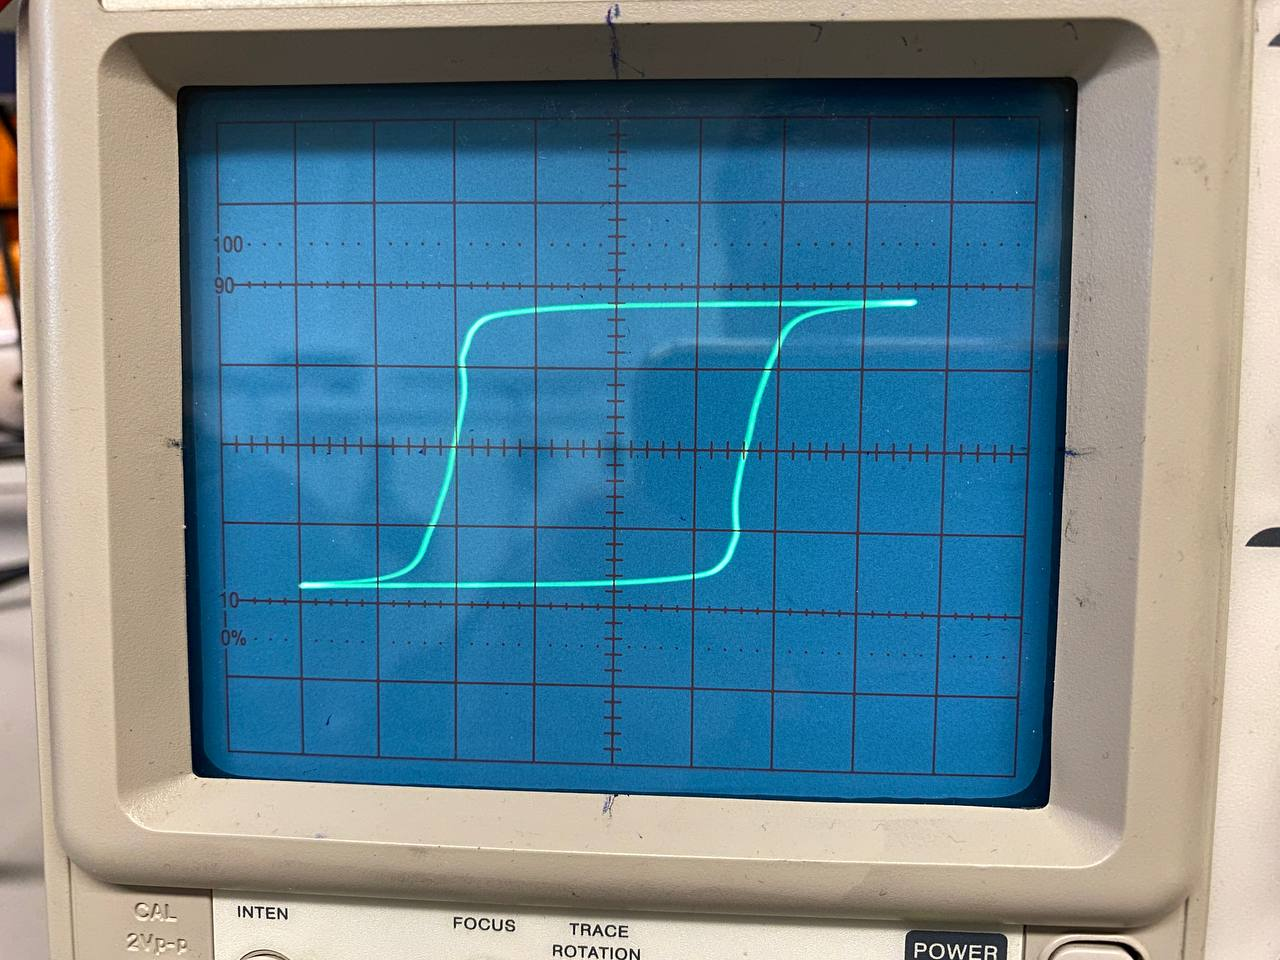
\includegraphics[width = 0.25\textwidth]{пермаллой.jpg}} &  \multicolumn{2}{c|}{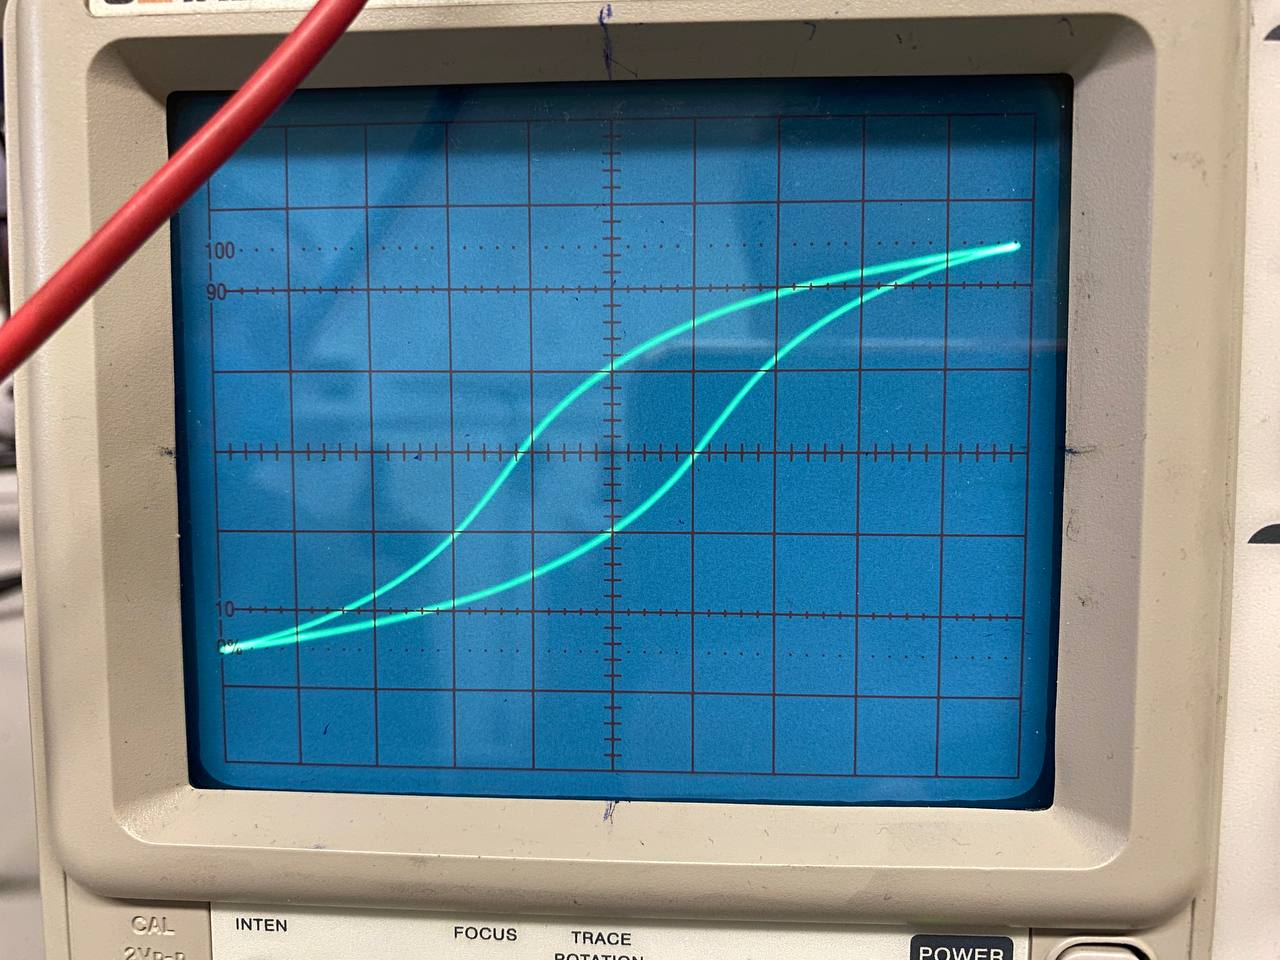
\includegraphics[width = 0.25\textwidth]{феррит.jpg}} &  \multicolumn{2}{c|}{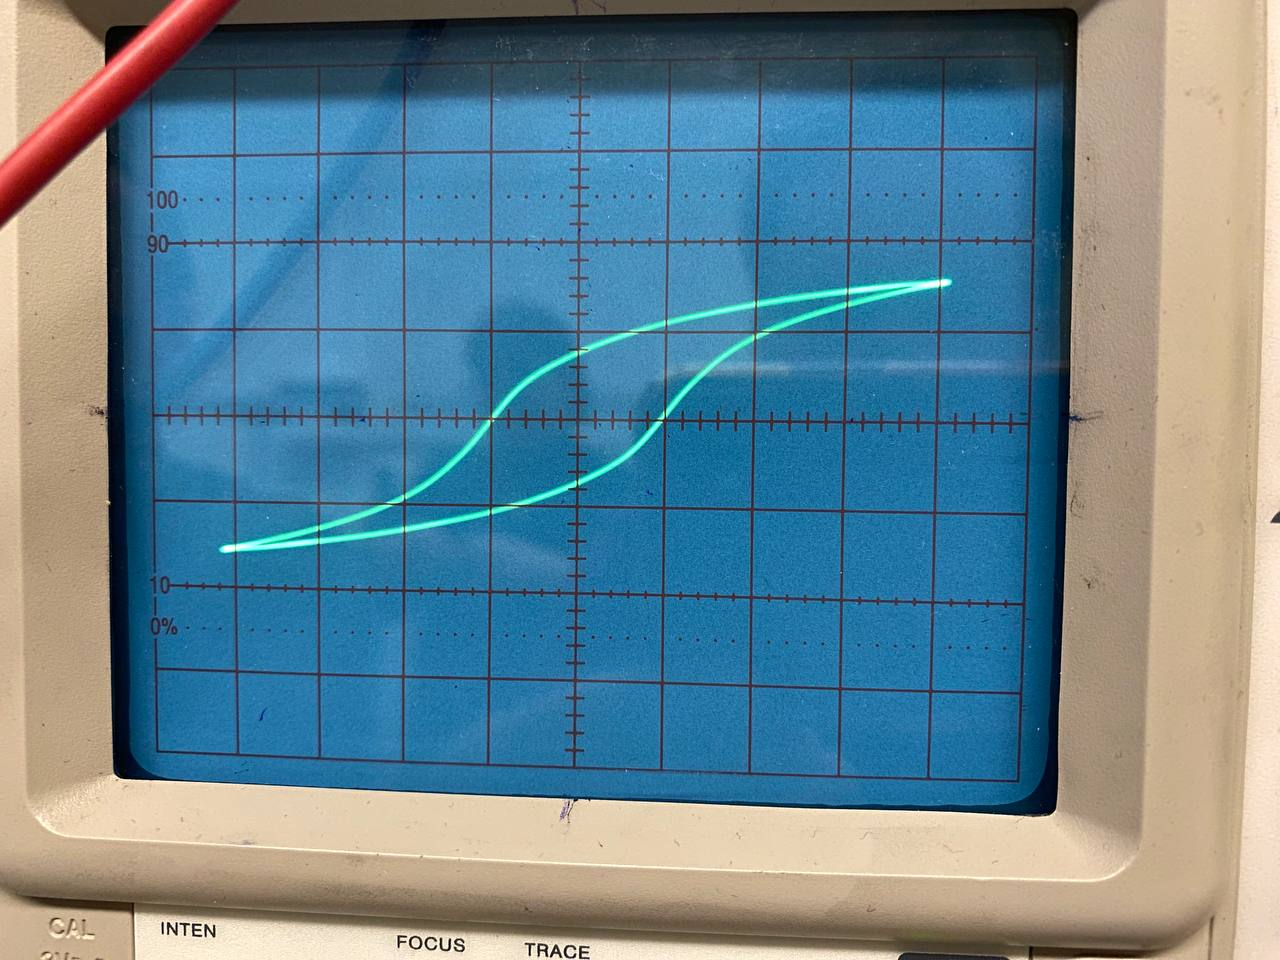
\includegraphics[width = 0.25\textwidth]{кремнистое железо.jpg}} \\ \hline
			$I_{\text{эф}}$, мА & 171.8 & 0.9 & 277 & 0.2 & 588 & 1 \\ \hline
			$[2x(c)]$, ед & 7.2 & 0,2 & 4.2 & 0,2 & 4.8 & 0,2 \\ \hline
			$[2y(r)]$, ед & 3,6 & 0,2 & 4 & 0,2 & 3.8 & 0,2 \\ \hline
			$K_x$ & 0,01 & 0 & 0,01 & 0 & 0,02 & 0 \\ \hline
			$K_y$ & 0,05 & 0 & 0,01 & 0 & 0,02 & 0 \\ \hline
			$H$, А/м & 7.5 & 0,02 & 8.4 & 0,2 & 22.7 & 0,3 \\ \hline
			$H_c$, А/м & 27 & 3 & 17.6 & 0.6 & 54.5 & 2.1 \\ \hline
			$B_r$, Тл/дел & 0.877 & 0,011 & 0.033 & 0,004 & 0,16 & 0,012 \\ \hline
			$B$, Тл & 1.57 & 0,13 & 0.066 & 0.012 & 0,31 & 0,02 \\ \hline
		\end{tabular}\\
		\caption{Данные, полученные из петли гистерезиса}
	\end{table}
	
	\begin{table}[H]
		\centering
		\begin{tabular}{|c|cc|cc|cc|}
			\hline
			& \multicolumn{2}{c|}{пермалой}      & \multicolumn{2}{c|}{феррит}         & \multicolumn{2}{c|}{железо}       \\ \hline
			& \multicolumn{1}{c|}{знач}  & $\sigma(x)$  & \multicolumn{1}{c|}{знач}   & $\sigma(x)$  & \multicolumn{1}{c|}{знач}  & $\sigma(x)$ \\ \hline
			2x(s) & \multicolumn{1}{c|}{7}     & 0.2   & \multicolumn{1}{c|}{9.6}    & 0.2   & \multicolumn{1}{c|}{8}     & 0.2  \\ \hline
			2y(s) & \multicolumn{1}{c|}{3.6}   & 0.2   & \multicolumn{1}{c|}{5}      & 0.2   & \multicolumn{1}{c|}{3}     & 0.2  \\ \hline
			$K_x$    & \multicolumn{1}{c|}{0.02}  & 0     & \multicolumn{1}{c|}{0.02}   & 0     & \multicolumn{1}{c|}{0.05}  & 0    \\ \hline
			$k_y$    & \multicolumn{1}{c|}{0.05}  & 0     & \multicolumn{1}{c|}{0.02}   & 0     & \multicolumn{1}{c|}{0.05}  & 0    \\ \hline
			$H$, А/м дел     & \multicolumn{1}{c|}{13.67} & 0.42  & \multicolumn{1}{c|}{16.8}   & 0.4   & \multicolumn{1}{c|}{56.8}  & 0.7  \\ \hline
			$H_s$, А/м   & \multicolumn{1}{c|}{47.85} & 0.2   & \multicolumn{1}{c|}{80.64}  & 0.41  & \multicolumn{1}{c|}{227.2} & 0.8  \\ \hline
		$B$, Тл/дел    & \multicolumn{1}{c|}{0.877} & 0.011 & \multicolumn{1}{c|}{0.067}  & 0.011 & \multicolumn{1}{c|}{0.4}   & 0.05 \\ \hline
		$B_s$, Тл   & \multicolumn{1}{c|}{1.58}  & 0.23  & \multicolumn{1}{c|}{0.1675} & 0.011 & \multicolumn{1}{c|}{0.6}   & 0.06 \\ \hline
		\end{tabular}
	\caption{Значения поля и индукции, амплитудное}
		\end{table}
	\subsection*{Калибровка оси X}
	Отключаем намагничивающую обмотку от цепи, соединив оба провода, идущих к обмотке, на одной из ее клемм. 
	
	Подбираем такой ток, чтобы горизонтальная прямая занимала большую часть экрана.
	
	Рассчитаем чувствительность канала $m_X$ по формуле $(3)$. 
	
	Результаты смотри в таблице 3.
	\subsection*{Калибровка оси Y}
	Разберем цепь. Соединим вход $Y$ с клеммами делителя "1/100-земля". Не меняя рабочего коэффициента $K_Y$, подберем с помощью трансформатора напряжение, при котором вертикальная прямая занимает почти весь экран. Измеряем длину $2y$. Запишем данные из двух вышеизложенных пунктов в таблицу. Рассчитаем $m_Y$ по формуле $(4)$.
	
	\begin{center}
		\begin{tabular}{|c|c|c|c|c|c|c|}
			\hline
			& Величина & $\sigma$ & Величина & $\sigma$ & Величина & $\sigma$ \\ \hline
			& \multicolumn{2}{c|}{Пермаллой} & \multicolumn{2}{c|}{Феррит 1000нн} & \multicolumn{2}{c|}{Кремнистое железо} \\ \hline
			$2x$, ед & 6,0 & 0,1 & 7,0 & 0,1 & 10,0 & 0,1 \\ \hline
			$m_X$, {[}B/дел{]} & 0,020 & 0,001 & 0,092 & 0,001 & 0,057 & 0,001 \\ \hline
			$U_{\text{эф}}$, В & 0,13 & 0,01 & 0,50 & 0,01 & 0,50 & 0,01 \\ \hline
			$2y$, ед & 8,0 & 0,1 & 7,0 & 0,1 & 7,0 & 0,1 \\ \hline
			$m_Y$, {[}B/дел{]} & 0,046 & 0,001 & 0,202 & 0,001 & 0,202 & 0,001 \\ \hline
			$K_x$ & 0,02 & 0 & 0,02 & 0 & 0,05 & 0 \\ \hline
			$K_y$ & 0,05 & 0 & 0,1 & 0 & 0,02 & 0 \\ \hline
		\end{tabular}\\
		\textbf{Таблица 4.} Калибровка осей осциллографа.
	\end{center}
	По таблице видим, что соответствующие $K$ и $m$ равны с точностью до погрешности.
	\subsection*{Расчет $\tau$ постоянной времени для цепочки}
	Считаем $U_{\text{вх}} = 2y \cdot K_y$ и $U_{\text{вых}} = 2x \cdot K_x$.
	
	Запишем все полученные данные в таблицу и посчитаем $\tau$ по формуле $(5)$ и через параметры установки.
	\begin{center}
		\begin{tabular}{|c|c|c|}
			\hline
			Величина & Значение & Ошибка \\ \hline
			$2y$, ед & 8,0 & 0,2 \\ \hline
			$K_y$, В/ед & 2 & 0 \\ \hline
			$2x$, ед & 6,2 & 0,2 \\ \hline
			$K_x$, В/ед & 0,02 & 0 \\ \hline
			$U_{\text{вх}}$, В & 16,0 & 0,2 \\ \hline
			$U_{\text{вых}}$, В & 0,124 & 0,002 \\ \hline
			$\tau$ из формулы, c & 0,41 & 0,02 \\ \hline
			$\tau$ из пар. уст., c & 0,40 & 0,02 \\ \hline
		\end{tabular}\\
		\textbf{Таблица 5.} Измерение $\tau$.
	\end{center}
	\subsection*{Замеры $\mu$}
	\begin{figure}[H]
		\centering
		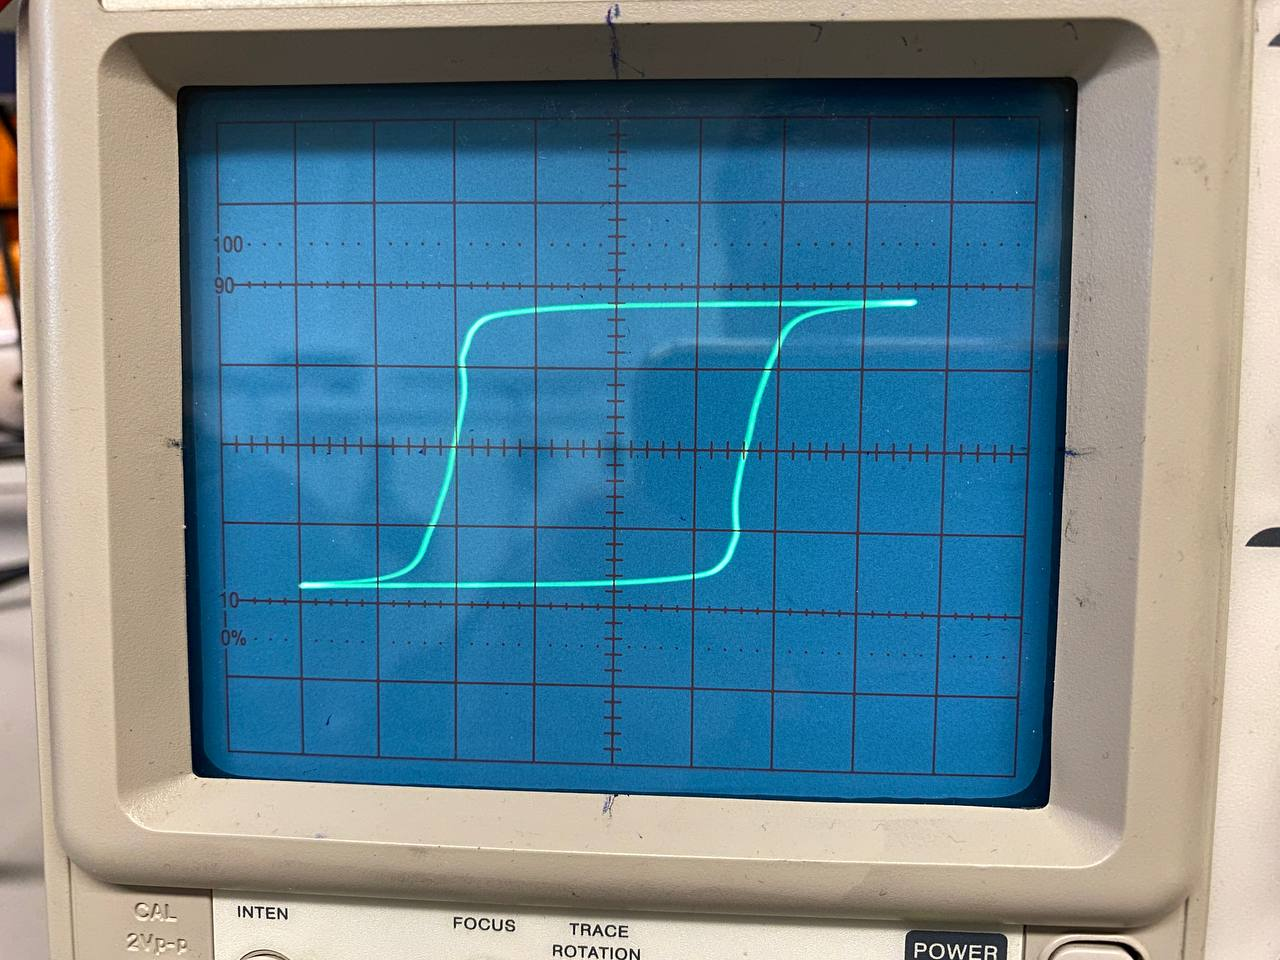
\includegraphics[width=0.8\linewidth]{пермаллой}
		\caption{Петля гистерезиса пермаллоя, с нанесенным участком убывания}
		\label{fig:}
	\end{figure}
	\begin{figure}[H]
		\centering
		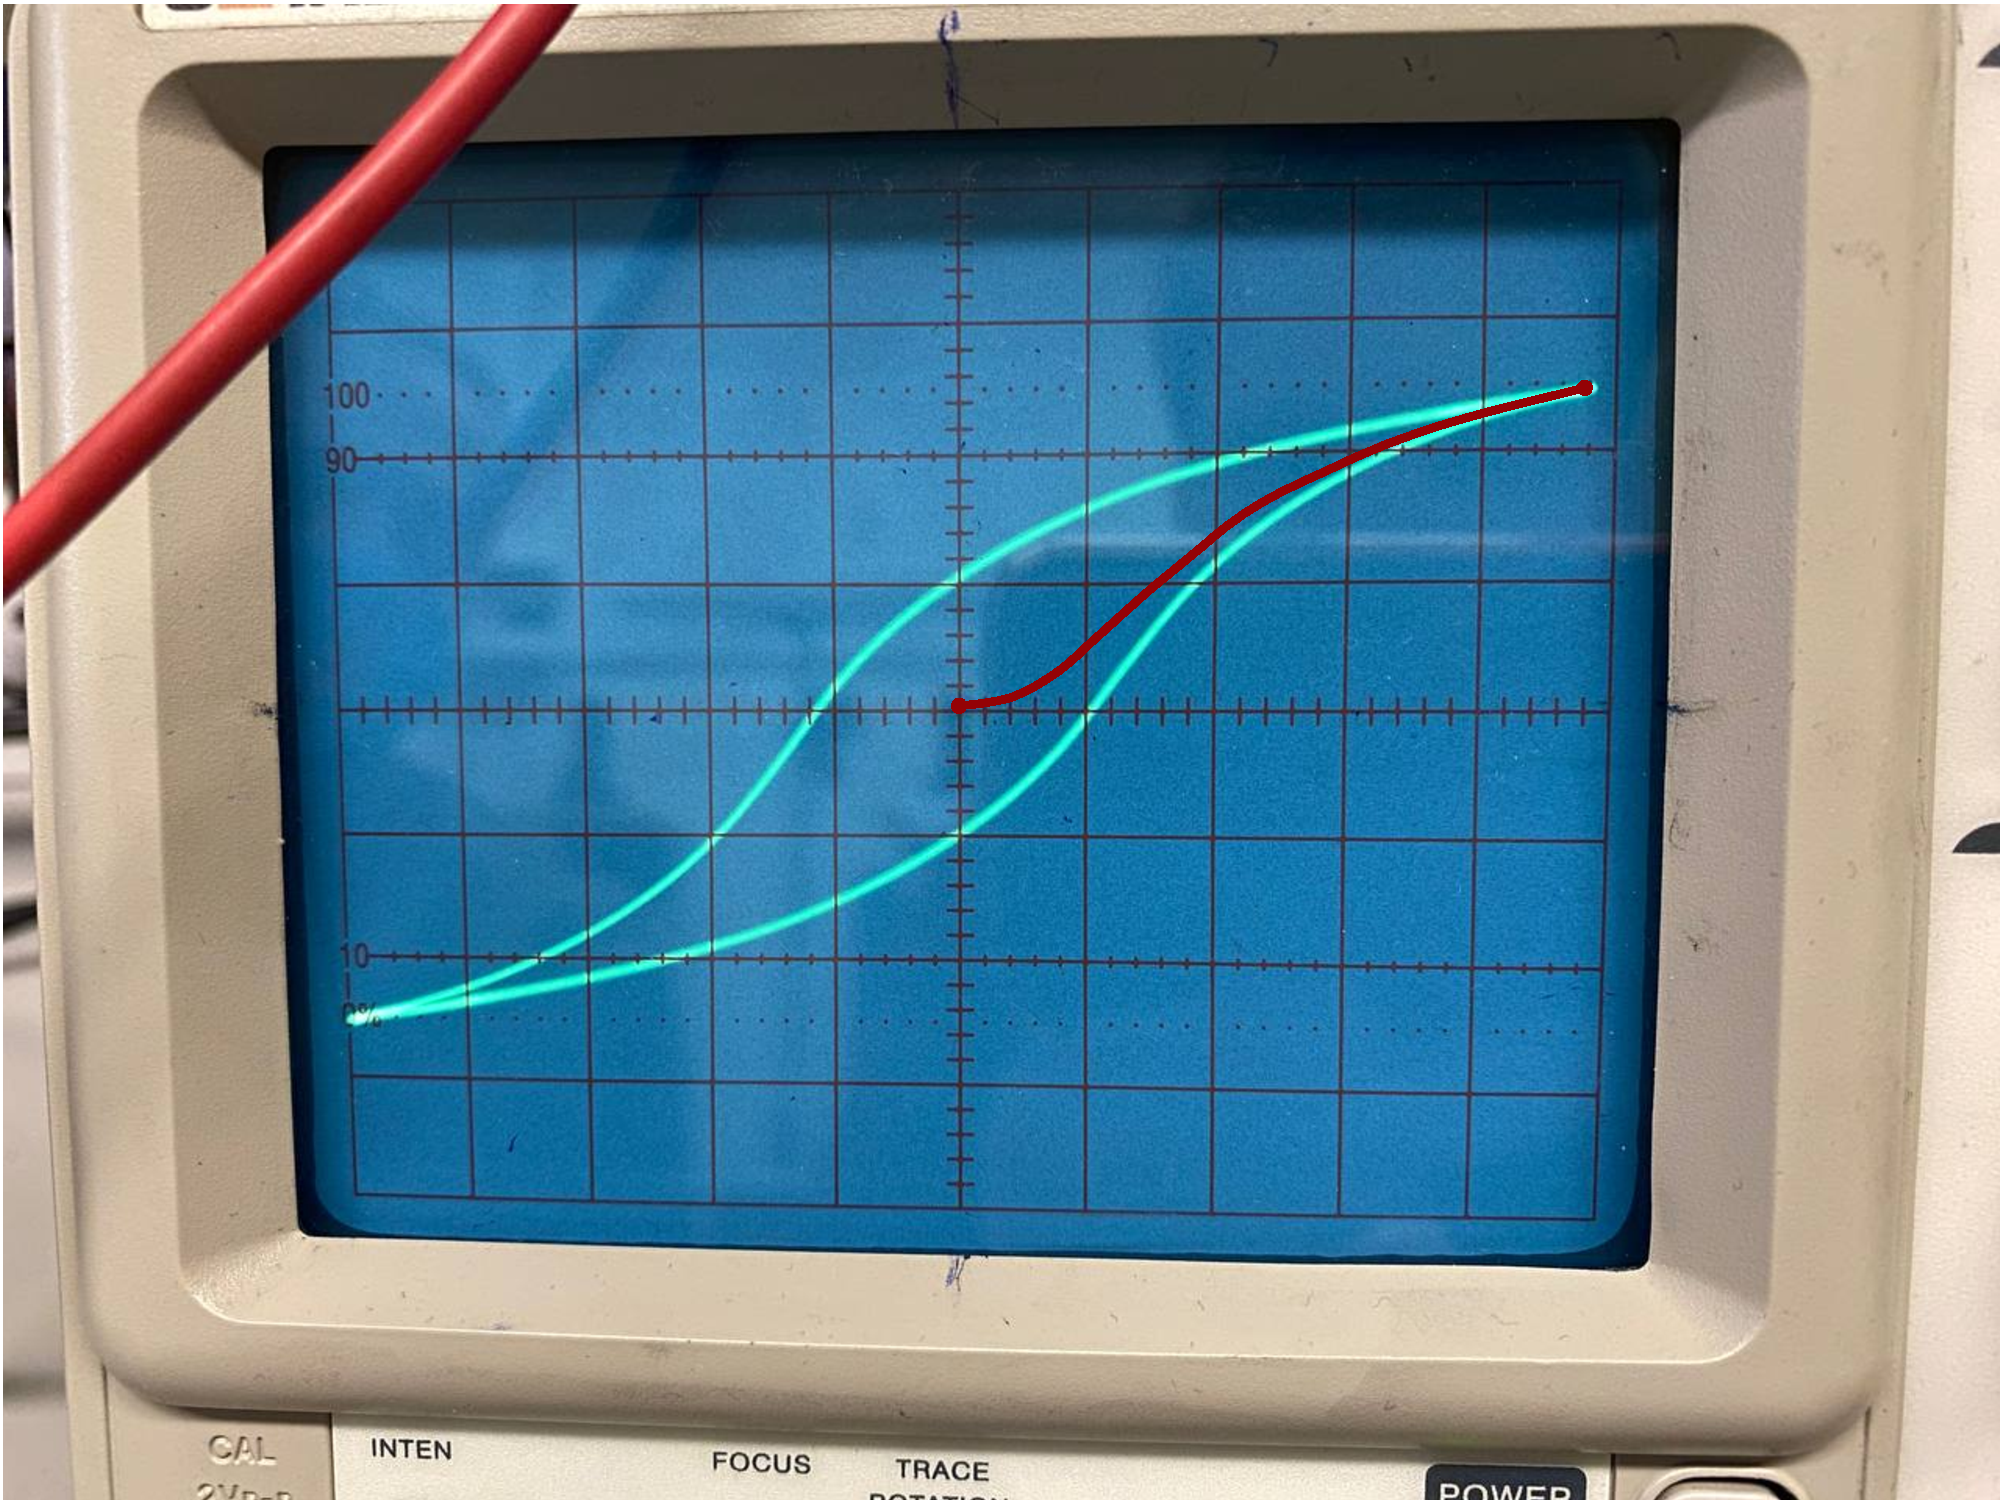
\includegraphics[width=0.8\linewidth]{феррит}
		\caption{Петля гистерезиса феррита, с нанесенным участком убывания}
		\label{fig:}
	\end{figure}
	\begin{figure}[H]
		\centering
		\includegraphics[width=0.8\linewidth]{"кремнистое железо"}
		\caption{Петля гистерезиса кремнистого железа, с нанесенным участком убывания}
		\label{fig:-}
	\end{figure}
	Замерить $\mu$ для пермаллоя не представляется возможным, так как в процессе изменения напряжения контура петля Гистерезиса принимала совершенно различные формы не дающие возможности оценить значение.\\
	Для феррита получаем: $\mu_{дифф}/\mu _0 =  6 * 10^3$\\
	Для кремнистого железа:  $\mu_{дифф}/\mu _0 =  8 * 10^3$\\
	\section{Выводы}
	1) Получили петли Гистерезиса для различных материалов.\\
	2) Оценили дифференциальную магнитную проницаемость для феррита и кремнистого железа.\\
	табличные значения: \\
	Для феррита: $\mu_{дифф}/\mu _0 =  5 * 10^3$\\
	Для кремнистого железа:  $\mu_{дифф}/\mu _0 =  6.3 * 10^3$\\
	3) Получили значения близкие к табличным, однако судить о погрешности достаточно сложно ввиду взятия угла наклона по картинке построенной по изменению петли на экране осциллографа.
	
	
\end{document}